\documentclass[conference]{IEEEtran}
\IEEEoverridecommandlockouts
% The preceding line is only needed to identify funding in the first footnote. If that is unneeded, please comment it out.
\usepackage{cite}
\usepackage{amsmath,amssymb,amsfonts}
\usepackage{algorithmic}
\usepackage{graphicx}
\usepackage{textcomp}
\usepackage{xcolor}
\usepackage{multirow}
\def\BibTeX{{\rm B\kern-.05em{\sc i\kern-.025em b}\kern-.08em
    T\kern-.1667em\lower.7ex\hbox{E}\kern-.125emX}}
\begin{document}

\title{Research Design 2:\\ Comparing Reinforcement Learning and Finite State Machine Agents in Real Time Strategy Games: Impact on Player Experience}

\author{\IEEEauthorblockN{Joshua Polanszky}
	\IEEEauthorblockA{\textit{Institute of Information Communication Technology} \\
		\textit{Malta College of Arts Science and Technology}}
	Paola, Malta
}

\date{\today}

\maketitle

\begin{abstract}
	In this study, we investigate the impact of Reinforcement Learning (RL) agents compared to traditional Finite State Machines (FSM)s on player experience.
	A simple Real-Time Strategy (RTS) game was developed to test whether RL agents provide a better player experience than FSMs. After a playtest with 2 
	groups of participants, we found that RL agents generally provided a more engaging and immersive experience, especially at higher levels of difficulty,
	while FSMs were preferred at easier levels. The results indicate that the development time and computational cost of RL agents may be justified in RTS games.
\end{abstract}

\begin{IEEEkeywords}
	Reinforcement Learning (RL), Finite State Machine (FSM), Real-Time Strategy (RTS) Games, Player Experience, Game AI
\end{IEEEkeywords}

\section{Introduction}

\subsection{Theme and Topic Rationale}

The Theme chosen is Decision-Making AI for Real-Time Strategy (RTS) Games, focusing on a direct comparison between traditional Finite State-Machine (FSMs) AI opponents against Machine Learning (ML) opponents,
specifically Reinforcement Learning (RL), and their impact on player experience. The rationale for this topic stems from the increasing standard of player expectations in games, and the need for more adaptive,
engaging AI opponents in games.

\subsection{Positioning and Research Onion}
This research addresses the gap in player experience found in the literature, being that while a lot of studies have been conducted on the performance or RL agents,
very few focused on the player experience difference between them, and FSMs. 
% By building on the works of \cite{grech_creating_2023} and \cite{vinyals_grandmaster_2019} on AlphaStar, this study will address the gap by
% providing a better understanding on the role RL agents will play in the future of RTS games. 
As can be seen in Figure \ref{fig:research_onion}, this study will follow a positivist research paradigm,
following a deductive and experimental approach, gathering both quantitative and qualitative data to measure player experience.

\begin{figure}[htbp]
	\centering
	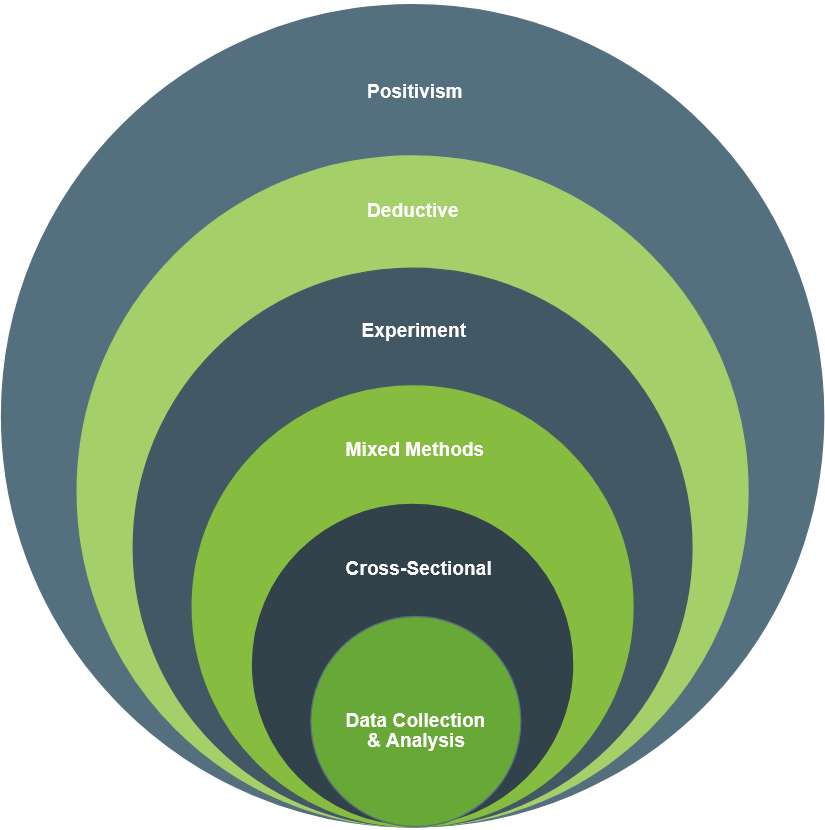
\includegraphics[width=0.4\textwidth]{Images/Research_Onion.PNG}
	\caption{Research Onion}
	\label{fig:research_onion}
\end{figure}


\subsection{Background to the Research Theme}

Game AI plays a huge role in player experience and immersion, as they provide the challenge and unpredictability that makes games fun and engaging.
It has evolved significantly over the years, especially in RTS games. Early RTS titles, such as StarCraft, relied on Finite State Machines (FSMs) for their AI decision-making \cite{vinyals_grandmaster_2019}. 
These FSM-based approaches, while simple and easy to implement, are deterministic and predictable, which can lead to repetitive and boring gameplay,
and allow players to exploit the gameplay patterns of the AI \cite{noauthor_finite_2020} \cite{jagdale_finite_2021}.

More recently, RL has emerged as an alternative AI approach, taking advantage of advancements in ML and computer hardware. In games such as AlphaStar \cite{vinyals_grandmaster_2019}, RL agents were able to
demonstrate adaptive and human-like behaviour, providing a more challenging and engaging experience for players. Another paper that highlights this is the work done by Grech \cite{grech_creating_2023},
where he created multiple difficulties of AI opponents using RL, and found that players reported higher levels of enjoyment and immersion. 
% Seems excessive for an introduction and background section, and most of these are already in the literature review.
% A similar study is the one done by \cite{bin_ramlan_implementation_2021},
% where they trained an RL agent to act as an opponent in a fighting game, with the agent being able to adapt to the player's skill level, and provide a more engaging experience, similar to the work done by \cite{vinyals_grandmaster_2019}

Despite all of this, the implementation of RL in commercial games remains limited due to the high computational cost, long training and development times, and added complexity.
This further proves the need for research in this area, and in evaluating if the benefits of RL agents in RTS games are worth the cost compared to traditional FSMs.

\subsection{Hypothesis}

Players report a higher level of enjoyment and improved experience when playing against RL agents compared to FSMs in RTS games.

\subsection{Independent \& Dependent Variables}

Independent variables are variables that are manipulated by the researcher and are mainly used to influence the dependent variables. 
Dependent variables are what happen because of the independent variables and are what the researcher is interested in measuring.

The independent variable in this study is the type of AI opponent. The dependent variables, those are player experience, player immersion, and perceived difficulty.
Player experience will be measured through surveys and engagement metrics, player immersion will be measured through surveys and validated game design principles, and perceived difficulty will be measured through
surveys, player feedback, and engagement metrics.

\subsection{Research Aim}

The aim of this study is to determine whether the use of Reinforcement Learning (RL) agents in Real-Time Strategy (RTS) games leads to a measurable improvement in player experience compared to traditional
Finite State Machine (FSM) opponents. Below are the specific research objectives:

\begin{itemize}
	\item Compare player-reported enjoyment, engagement, and immersion levels when playing against RL and FSM AI opponents in RTS games.
	\item Identify the key factors influencing player experience for each AI approach.
	\item Determine if the computational and development costs and complexity of RL are justified in RTS games.
\end{itemize}

\subsection{Purpose Statement}

This study is important because AI opponents shape the core gameplay experience of RTS games. The adaptiveness and human-like behaviour of RL agents have the potential to
significantly enhance player experience, if implemented correctly.

By investigating the difference in player experience between RL and FSM AI, this study will provide valuable insights to game developers, AI designers, and the broader gaming community, helping them
in making more informed decisions regarding AI decision-making strategies in RTS game development.

\section{Literature Review}

The difference between academic and non-academic literature is that academic literature is peer-reviewed, and is as such, more reliable and trustworthy
than non-academic literature, which can easily be biased or contain false information. Academic literature can also be more in-depth and detailed, due to
the high research standards and requirements of academic institutions, especially IEEE.

\begin{figure}[htbp]
	\centering
	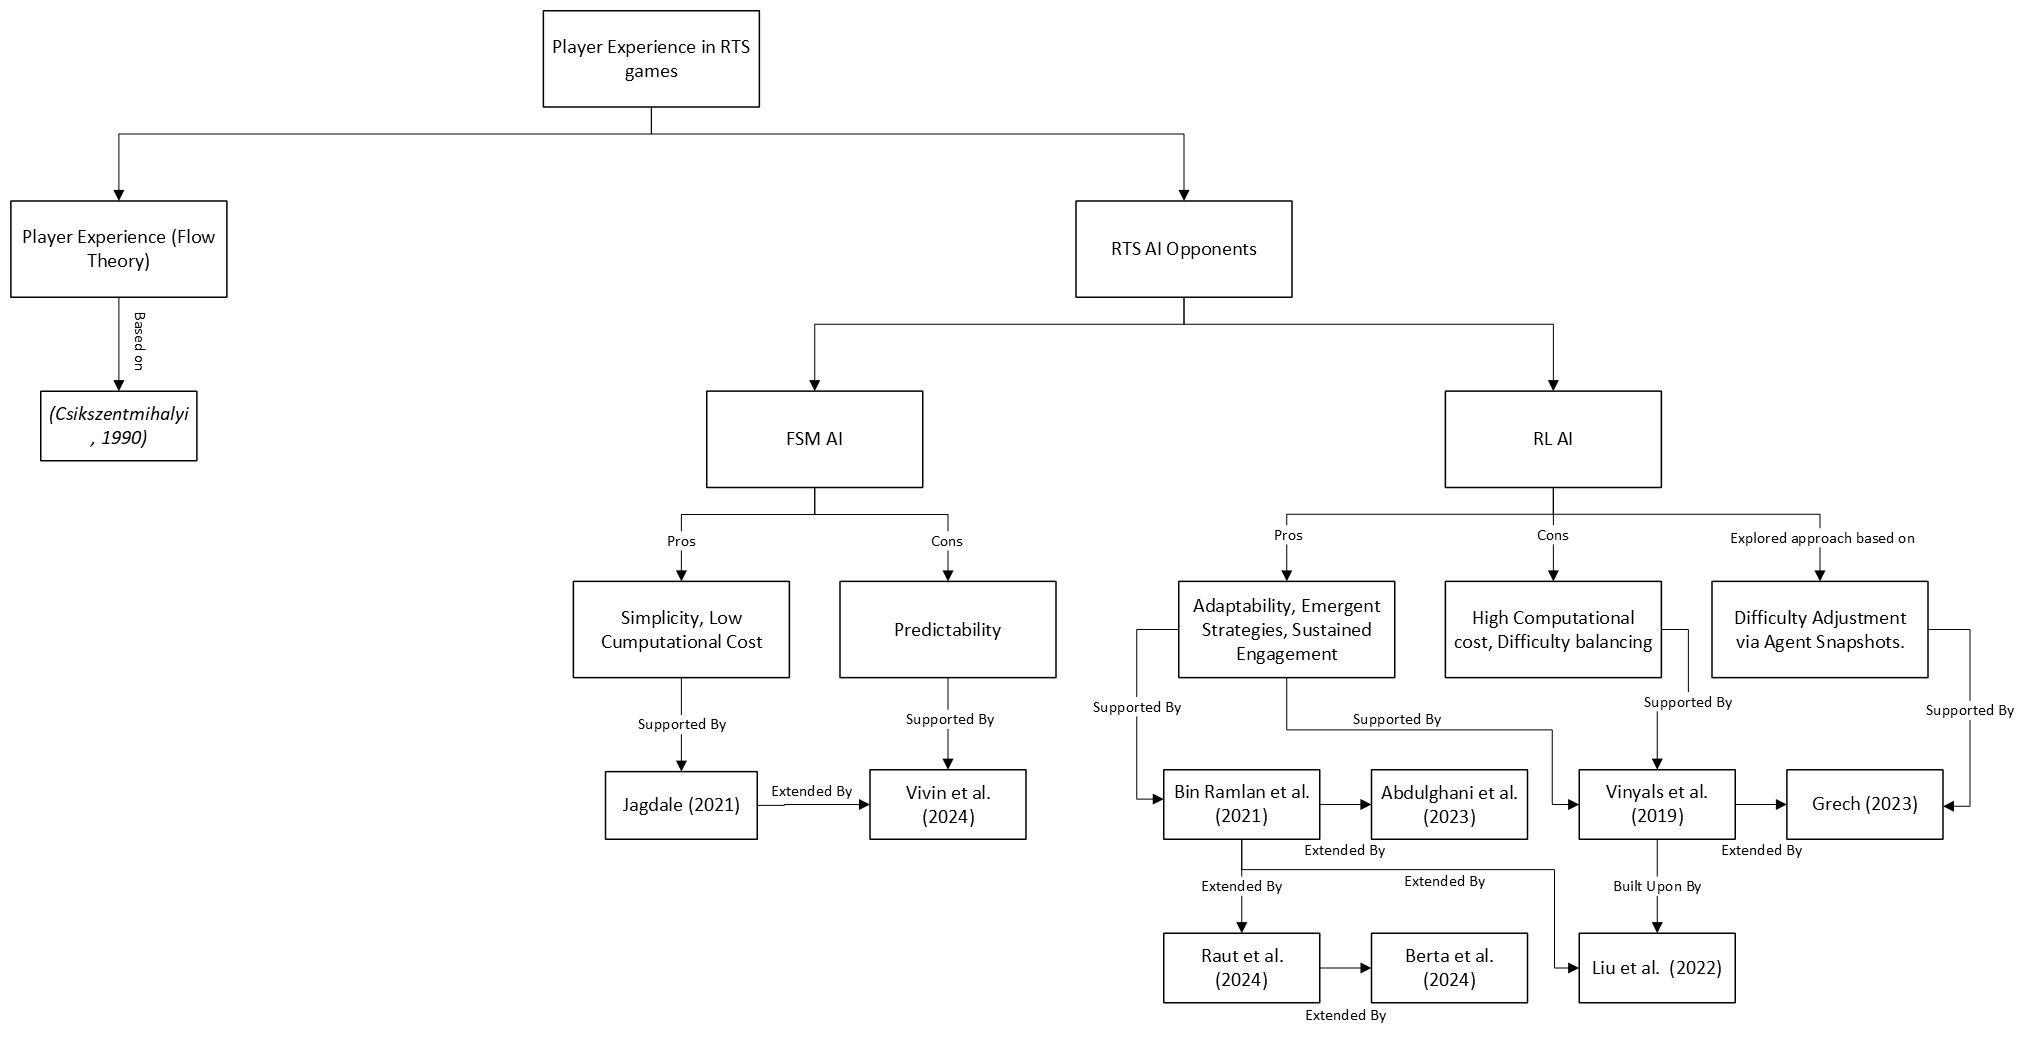
\includegraphics[width=0.45\textwidth]{Images/Literature_Map.png}
	\caption{Literature Map}
	\label{fig:literature_map}
\end{figure}

The goal of a game developer is to create a game that is fun and engaging, and they achieve this by creating a game that is both challenging and rewarding, without being too difficult or frustrating.
This leads into the concept of player experience, which is a subjective measure of how much a player enjoys a game, and is influenced by many factors. One of the most influential frameworks for understanding player
experience is Csikszentmihalyi's flow theory \cite{csikszentmihalyi_flow_1990}, which describes a mental state in which a player is fully immersed, focused and involved in the game, leading to an improved sense of
enjoyment and intrinsic motivation. According to Csikszentmihalyi, flow occurs when the challenges presented match the player's skill level, and multiple conditions must be met for players to enter this state.
These are having clear goals, and immediate feedback, and when these conditions are met, players are more likely to lose track of time and become deeply immersed in the game world \cite{csikszentmihalyi_flow_1990}.

AI opponents play a critical role in maintaining this balance, as they provide the challenge and difficulty that the player must overcome. Traditionally FSMs are used for this, as they are simple to implement
and easy to understand, and when done correctly, provide a good challenge to the player. However, given enough time, players can learn the patterns of the FSMs, and exploit them,
making the game feel boring and leading to them falling out of the \textit{flow state} \cite{noauthor_comparative_nodate}. It is possible to combat this through weakening the player, or making the AI more difficult,
as is done in Souls-like games, however this can prove too challenging and overwhelm the player, as well as making the perceived balance seem unfair, once again breaking the flow \cite{jagdale_finite_2021} \cite{noauthor_finite_2020}.

RL agents, on the other hand, are able to learn how to play the game, and as such, adapt to the player and given scenario. This creates a more engaging
and immersive experience, as the player feels like they are playing against a real opponent, and not just a computer. This is especially true in RTS games,
due to the complexity of the game, and the many strategies that can be taken, which can be seen in the works done by \cite{vinyals_grandmaster_2019} and \cite{grech_creating_2023}.
A common tool used in most of these papers is the Unity ML-Agents toolkit, which is a framework for training RL agents in Unity games, making it easier to implement and train RL agents for research purposes.
Along with that, most used the Proximal Policy Optimization (PPO) algorithm, which is a popular RL algorithm that is used for training agents in continuous action spaces, which is especially useful in real-time games.

In the work done by \cite{vinyals_grandmaster_2019}, they trained an RL agent to play StarCraft II, and found that the agent was able to not only learn how to play the game, but also adapt to the player's actions and strategies in real time.
A similar result was found in the works done by \cite{bin_ramlan_implementation_2021} and \cite{raut_unity_2024}, where both used the Unity ML-Agents toolkit with PPO to train RL agents in 2 different genres.
\cite{bin_ramlan_implementation_2021} trained an RL agent to play a fighting game, with rewards for moving closer to the player, landing attacks and winning, and penalties for being hit, missing and losing.
\cite{raut_unity_2024} trained an RL agent to play a racing game, with the reward structure being based on the distance travelled and the time taken, which punishes the agent for crashing and/or taking too long.
Combined, these 3 papers show the power of RL agents in real-time games, and their adaptability to the player, however they all share the same 2 flaws. The agents are computationally expensive to train, and to
run, requiring a lot of time and resources not only for the developers, but also the players as they need to have a powerful enough computer to run the game and agent simultaneously. Along with that, the agents
can become too difficult to play against, and as such break the flow state, as the player is unable to keep up with the agent's actions and strategies, especially if they are new to the game.

\cite{grech_creating_2023} tackled this issue by saving multiple snapshots of the agent during training and using them to create different difficulties of AI opponents, similarly to how FSM difficulties are created.
Their results showed that players reported higher levels of enjoyment and immersion when playing against the RL agents, just like the previous works, with the key difference that new players were also able to enjoy
the game. Their implementation was rather simple, and as such requires more research to be done in improving it and identifying if it is a viable solution to the issues of RL agents. Another option would be
to build in a dynamic difficulty adjustment (DDA) system into either the agent or the game, as suggested by \cite{grech_creating_2023}, which would keep the rl agent's difficulty in check, while keeping its
adaptability and unpredictability. This shows the gap in literature, both in the comparison of RL and FSM AI opponents, but also in managing the difficulty of RL agents.

% Wouldnt just having them in the references section be enough?
\subsection{Further Reading}

% Takes up too much space, and most are found in the references section anyway.
\begin{itemize}
	\item Grech G. (2023). \textit{Creating Difficulty Levels with Reinforcement Learning in a Strategy Game}. \cite{grech_creating_2023}
	\item Raut, U., Galchhaniya, P., Nehete, A., Shinde, R., \& Bhoite, A. (2024). \textit{Unity ML-Agents: Revolutionizing Gaming Through Reinforcement Learning}. \cite{raut_unity_2024}
	\item Bin Ramlan, A. A., Ali, A. M., Abdul Hamid, N. H., \& Osman, R. (2021). \textit{The Implementation of Reinforcement Learning Algorithm for AI Bot in Fighting Video Game}. \cite{bin_ramlan_implementation_2021}
	\item Liu, R.-Z., Pang, Z.-J., Meng, Z.-Y., Wang, W., Yu, Y., \& Lu, T. (2022). \textit{On Efficient Reinforcement Learning for Full-length Game of StarCraft II}. \cite{liu_efficient_2022}
	% \item Abdulghani, A. M., Abdulghani, M. M., Walters, W. L., \& Abed, K. H. (2023). \textit{Multi-Agent Reinforcement Learning System Using Value-Decomposition Network Algorithm in StarCraft Environment}. \cite{abdulghani_multi-agent_2023}
	\item Vinyals, O., Babuschkin, I., Czarnecki, W. M., et al. (2019). \textit{Grandmaster level in StarCraft II using multi-agent reinforcement learning}. \cite{vinyals_grandmaster_2019}
	% \item Berta, R., Lazzaroni, L., Capello, A., et al. (2024). \textit{Development of Deep-Learning-Based Autonomous Agents for Low-Speed Maneuvering in Unity}. \cite{berta_development_2024}
	\item Jagdale, D. (2021). \textit{Finite State Machine in Game Development}. \cite{jagdale_finite_2021}
	% \item \textit{Comparative Analysis of Game Development Techniques: Using Finite State Machine, Physics Simulation, Path Finding, Event Handling}. \cite{noauthor_comparative_nodate}
\end{itemize}

\section{Research Methodology}

\subsection{Research Questions}
The research questions for this study are:

\begin{enumerate}
	\item How do RL and FSM AI opponents compare in terms of player experience in RTS games?
	\item What are the key factors that influence player experience when playing against RL and FSM AI opponents in RTS games?
	\item How do RL and FSM AI opponents impact player immersion in RTS games?
\end{enumerate}

\subsection{Research objectives}

The objective for the research is to evaluate the impact of RL and FSM opponents in RTS games, and to determine their impact on player experience and immersion,
and what are the key factors that cause this impact/influence. This is to be done by creating a simple RTS game, and implementing both RL and FSM agents,
and then conducting a play test experiment with players, where both groups will then be surveyed to gather data on their experience. Along with this,
data gathered during the playtest through unity analytics will be used to measure player engagement and immersion.

\subsection{Suitable Methodology}

This study adopts a \textbf{positivist research philosophy}, which means it emphasizes the use of objective measurements and observable phenomena, and it is suitable for this study as it aims
to evaluate the impact of RL and FSM AI opponents on player experience through measurable data, aligning it with \textbf{quantitative methodology}. It follows a \textbf{deductive approach}, with an \textbf{experimental research design},
as it starts with a hypothesis, and then using an experimental prototype, tests the hypothesis by allowing participants to play it, and then uses the data to observe the difference the independent variable (AI type)
has on the dependent variables \textbf(player experience, immersion, and perceived difficulty). This will then be used to answer the research questions and prove the hypothesis. It is important to note that the study
will also gather an fair amount of qualitative data, making it a \textbf{mixed-methods approach}. This is done to help align the more human aspects of player experience with the more quantitative aspects.

\subsection{Description of methodology, design, and approach}

A simple RTS game was created, using both RL and FSM agents, and a deductive experiment was conducted. The players were split into 2 groups,
where the first group played against the FSM first, then RL, across all difficulties, and the second group did the same, but with RL first.
After each difficulty, they were asked to fill out a questionnaire with quantitative and open-ended questions about their experience.
The qualitative data will help capture the more human aspects of player experience, and along with in-game analytics and logs, 
will be used to validate the data gathered from the questionnaires. This will help in answering the research questions, and keep everything measurable and comparable.

\subsection{Reflection on validity and reliability of the research design}

\textbf{Validity}: The study ensures validity by designing the experiment to control for confounding variables, such as the order in which participants play, since on the second playtest they would be more
familiar with the game mechanics and controls. The use of validating the survey results with in-game analytics and engagement metrics further strengthens the validity of the research being conducted.

\textbf{Reliability}: To help ensure reliability, the same setup, game environment and surveys will be used for all participants. Any and all instructions will be standardised, using text and/or video/audio
recordings to ensure that all participants are given the same instructions, without any bias that comes from the researcher. All data collection processes will be automated, further standardising the process
and ensuring reliability.

\textbf{Generalizability/Transferability}: While the finding will be focused on the specific RTS game developed for this study, the insights gained can be generalised to other games within the RTS genre,
which follow similar game mechanics. The results may also be applicable to other game genres with similar AI opponent implementations, such as turn-based strategy games, but the transferability
of results could be limited, and as such should be explored in future research.

\subsection{Ethical considerations}

Since the playtest will not be conducted on minors, and will not involve any sensitive or identifiable data, the main ethical considerations
would fall onto the type of content in the game, and if it is appropriate for the players. In this case, it will be a simple cartoon like game,
so there should not be any issues with this. The participants will be informed of the nature of the game and the study, and be required to
sign a consent form before participating, and will be free to withdraw at any time.

\section{Findings and Discussion}

\subsection{Chapter Overview}
Following the prototype testing, the data collected from the playtest sessions was analysed to evaluate the impact of RL and FSM agents on player experience.
The analysis focused on comparing quantitative metrics such as player enjoyment, engagement, and immersion, and aligning them with the qualitative feedback as well as the in-game analytics.
This was done as to provide a more comprehensive understanding of player experience, and to identify the key factors that influence it.

\subsection{Findings}

Below are the average results from the playtest sessions, comparing player performance against both FSM and RL agents across three difficulty levels: easy, medium, and hard.

\begin{table}[h]
	\centering
	\caption{Average Player and Agent Scores, Win Rate, Engagement, and Immersion by Difficulty}
	\label{tab:results}
	\begin{tabular}{lcccccc}
		\hline
		\multirow{2}{*}{\textbf{Metric}} & \multicolumn{2}{c}{\textbf{Easy}} & \multicolumn{2}{c}{\textbf{Medium}} & \multicolumn{2}{c}{\textbf{Hard}}                           \\
		                                 & FSM                               & RL                                  & FSM                               & RL     & FSM    & RL    \\
		\hline
		Player Avg. Score                & 470                               & 489                                 & 540                               & 525    & 584    & 560   \\
		Agent Avg. Score                 & 390                               & 364                                 & 413                               & 460    & 433    & 520   \\
		Player Win Rate                  & 95\%                              & 100\%                               & 90\%                              & 85\%   & 85\%   & 70\%  \\
		Avg. Score Diff. (\%)            & 17.0\%                            & 24.4\%                              & 22.4\%                            & 12.4\% & 25.5\% & 7.1\% \\
		Enjoyment (1-5)                  & 3.9                               & 3.7                                 & 4.1                               & 4.2    & 4.0    & 4.5   \\
		Engagement (1-5)                 & 3.0                               & 2.9                                 & 3.2                               & 3.8    & 3.3    & 4.2   \\
		Immersion (1-5)                  & 2.9                               & 2.8                                 & 3.0                               & 3.7    & 3.1    & 4.1   \\
		\hline
	\end{tabular}
\end{table}

\subsection{Discussion of Results}

As we can see in Table \ref{tab:results}, on the easiest difficulty, players had a higher average score and win-rate against RL agents, with a win rate of 100\%, compared to 95\% against FSM agents.
In medium and hard difficulties however, RL agents were more competitive, with the average score difference decreasing significantly, and the player win rate dropping to 85\% and 70\% respectively.
This indicates that the split in difficulty levels was greater for RL agents, as the easy difficulty was easier, and the hard difficulty was harder, compared to FSM opponents.

We can also see that the score difference while higher for RL agents at easy difficulty, was a lot lower on the higher difficulties. This indicates that RL agents were able to adapt better,
and remained more consistent in their performance, while FSM agents were more predictable and less adaptive.

Regarding player enjoyment, we can see that like with the RL performance, players enjoyed FSMs more at the easy difficulty, while RL agents were more enjoyable at the medium and hard difficulties.
The same trend happens with engagement and immersion, with RL agents achieving an even greater increase in engagement and immersion compared to FSMs on the medium and hard difficulties,
with the gap in easy difficulty being smaller.

This suggests that the tougher the opponent, the more engaging and immersive the experience became, aligning with the findings of \cite{grech_creating_2023} and \cite{vinyals_grandmaster_2019}.
As for enjoyment, while it did increase with the harder difficulties, likely due to it being more engaging and immersive, it was not as pronounced as the other two metrics, indicating that the increased
loss rate and difficulty may have led to some frustration for players, especially with RL agents at the hard difficulty.

This aligns pretty well with the qualitative feedback gathered from the participants, where most players reported that the increased challenge and adaptability of RL agents made the game more engaging and fun,
with a few mentioning that the increased difficulty sometimes made it feel unfair. They compared this to feeling like an unbalanced match, where the skill difference was too great.
On the hard difficulty especially, a lot of feedback was given that the FSM agents were becoming easier, as while they were faster and making smarter decisions, it was clear what logic they were following,
and as such, some of the players were able to predict their actions and exploit them. This could help explain the higher average score difference for FSM agents at the hard difficulty, as players had learned
how to exploit it.

When aligning this with the hypothesis, we can see that it is partially supported, as while players on average reported higher levels of enjoyment and immersion when playing against RL agents,
this was only true at the medium and hard difficulties, with the easy difficulty being more enjoyable against FSM agents. This could have been due to the FSM agents being new to the players, and as such they
had not yet learned how to exploit them. This aligns well with the average score difference in Table \ref{tab:results}, where the score difference for FSMs was lowest at the easy difficulty.

The small sample size of participants, along with the results show above indicate that the reliability of the results might be slightly skewed,
as due to having them replay the game multiple times, they were better able to learn the patterns of the FSM agents, especially on the 3rd playthrough,
which was the hard difficulty. This, along with the fact that its a single game, could limit the generalisability of the results,

\subsection{Summary of Findings}
From the analysis of the playtest data, we saw that on easy difficulty, FSM agents provided a more meaningful challenge, and a better player experience than RL agents.
This could have been due to players not having learned how to exploit the FSM agents yet, or the RL agent being too inconsistent at this difficulty.
As the difficulty increased, RL agents became more competitive, with the average score difference decreasing significantly, and player experience metrics such as engagement and immersion increasing.
Contrarily, FSMs became more predictable and easier to exploit, leading to a decrease in player engagement and immersion at higher difficulties.
This means that hypothesis is only partially supported, as while players reported higher levels of enjoyment and immersion when playing against RL agents, this was not the case at the easy difficulty.

\section{Conclusion}

This study set out to compare the impact of Reinforcement Learning (RL) and Finite State Machine (FSM) agents on player experience in Real-Time Strategy (RTS) games.
The results from the playtest sessions indicate that in most cases, RL agents provide a more engaging and immersive experience for players.

The research questions were answered as follows: 
(1) RL agents generally outperformed FSMs in terms of player engagement at higher difficulty levels, while FSMs were preferred at easier levels; 
(2) The key factors influencing player experience between the two AI approaches were agent adaptability, predictability, and challenge;
(3) RL agents greatly improve player immersion, especially as difficulty increases, due to their adaptability and unpredictability, while FSMs suffered from predictability and were exploited by players;

As stated in the findings and discussion, the hypothesis was only partially supported, as players reported an improved experience when playing against RL agents
on all difficulties except for easy, where FSMs were preferred.

The limited number of participants and a more simplistic game design are the key limitations of this study, as the majority of participants were familiar with the game genre.
This likely influenced their ability to exploit the FSM agents, and made harder difficulties more desirable, as it better matched their skill level. This paired with having to replay the game multiple times on
harder difficulties may have skewed the results and their reliability. As for generalisability, due to it being a small scale study with a single simple game, the results may not be applicable to other RTS games,
or similar genres.

For future research, it is recommended to conduct a larger scale study with a more diverse player base, and to integrate Dynamic Difficulty Adjustment (DDA) systems to better balance the difficulty of the game.
This will help ensure that the game remains challenging across all skill levels, and remove the bias of having players repeat the game multiple times, increasing the difficulty each time.
Another recommendation is to explore the use of RL agents in other game genres, such as first-person shooters or action-adventure games, to see if the findings of this study can be generalised to other genres.

\bibliographystyle{ieeetr}
\bibliography{references}
\end{document}
